\naslov{Dinamika realnih funkcij}

\podnaslov{Osnovni pojmi}

Za začetek se bomo omejili na funkcije $f: I \to I$, kjer je $I$ interval v
$\R$.
Obravnavali bomo zaporedja $x_{n+1} = f(x_n)$ pri različnih začetnih pogojih
$x_0 \in I$.
Uvedimo oznako
\[
  f^n = \underbrace{f \circ f \circ \cdots \circ f}_{\text{$n$ pojavitev $f$}}.
\]

\begin{definicija}
  \pojem{Orbita} točke $x_0$ pri funkciji $f$ je množica
  $O_f(x_0) = \{ f^n(x_0) \such n \in \N_0 \}$.
  Množici vseh orbit za $x_0 \in I$ pravimo \pojem{dinamika funkcije $f$}.
\end{definicija}

\begin{primer}
  Za $x_{n+1} = x_n^2 + 1$ je orbita točke $1$ enaka $\{ 1, 2, 5, 26, \ldots \}$.
\end{primer}

Orbite lahko (za funkcije ene spremenljivke) vizualiziramo s
\pojem{pajčevinastim diagramom} (angl.~\textit{cobweb diagram}), prikazan na
sliki~\ref{fig:ds-02-pajcevinasti-diagram}.

\begin{figure}[h!]
  \centering
  {
  \newcommand{\startv}{.8}
  \begin{tikzpicture}[scale=5,declare function={f(\x)=\x*\x*\x;}]
	\draw[<->](0,1.1)|-(1.1,0);
	\draw[green!70!black] (0,0)--(1,1);
	\draw[blue, domain=0:1, smooth] plot (\x,{f(\x)});
	\foreach \t[evaluate=\t as \newv using f(\startv)] in {1,...,4}{
	  \draw[red] (\startv,\startv)|-(\newv,\newv);
	  \xdef\startv{\newv}
	}
  \end{tikzpicture}
  }
  \caption[Pajčevinasti diagram]{Pajčevinasti diagram za $f(x) = x^3$ z začetno
	točko $x_0 = 0.8$.\footnotemark{}}%
  \label{fig:ds-02-pajcevinasti-diagram}
\end{figure}

\footnotetext{Prirejeno po:
  \href{https://tex.stackexchange.com/questions/640022/how-to-draw-a-cobweb-graph-like-this-one}{stackexchange}}

\begin{definicija}
  Točka $x_0$ je \pojem{periodična} s periodo $n \in \N$ za $f$, če zanjo velja
  $f^n(x_0) = x_0$ in je $n$ najmanjše število s to lastnostjo.
  Če je $n = 1$, taki točki pravimo \pojem{fiksna točka}.
\end{definicija}

\begin{primer}
  Funkcija $f(x) = -x^3$ ima le eno fiksno točko, $0$.
  Izračunamo lahko, da imamo tudi dve točki periode $2$, to sta $1$ in $-1$.
\end{primer}

\begin{definicija}
  Orbiti $n$-periodične točke pravimo \pojem{$n$-cikel}.
\end{definicija}

\begin{definicija}
  Naj bo $x_0 \in I$ fiksna točka za $f: I \to I$.
  \begin{itemize}
  \item Točka $x_0$ je \pojem{šibko privlačna}, če obstaja okolica $U \ni x$, da
	za vsak $y_0 \in U$ velja $y_n = f^n(x_0) \to x_0$.
	Okolici $U$ pravimo \pojem{območje privlaka} za $x_0$, največjemu intervalu
	znotraj $U$ pa \pojem{neposredno območje privlaka} za $x_0$.
  \item Točka $x_0$ je \pojem{šibko odbojna}, če obstaja okolica $U \ni x$, da
	za vsak $y_0 \in U \setminus \{x_0\}$ obstaja $m \in \N$, da $f^m(y_0)
	\notin U$.
  \end{itemize}
\end{definicija}

\begin{definicija}
  Če je $f$ zvezno odvedljiva, uvedemo dodatne pojme. Točka $x_0$ je
  \pojem{privlačna}, če je $\abs{f'(x_0)} < 1$, \pojem{odbojna}, če je
  $\abs{f'(x_0)} > 1$, oziroma \pojem{nevtralna}, če je $\abs{f'(x_0)} = 1$.
\end{definicija}

\begin{primer}
  Funkcije $f_1(x) = x+x^3$, $f_2(x) = x - x^3$ in $f(x) = x + x^2$ imajo vse
  fiksno točko v $0$, a se obnaša drugače.
  V prvem primeru je $0$ šibko odbojna točka, v drugem šibko privlačna, v zadnjem pa
  niti ena niti druga.
  Preverimo lahko, da je v vseh primerih $\abs{f_i'(0)} = 1$, torej so vse točke
  odbojne.
\end{primer}

\begin{figure}[h!]
  \centering
  \begin{subfigure}{0.3\textwidth}
	\centering
	\begin{tikzpicture}[scale=1.9,declare function={f(\x)=\x*\x*\x+\x;}]
	  \draw[<->](0,1.1)|-(1.1,0);
	  \draw[<->](0,-1.1)|-(-1.1,0);
	  \draw[green!70!black] (-1,-1)--(1,1);
	  \draw[blue, domain=-0.7:0.7, smooth] plot (\x,{f(\x)});
	\end{tikzpicture}
	\caption{$f_1(x) = x + x^3$}
  \end{subfigure}
  \begin{subfigure}{0.3\textwidth}
	\centering
	\begin{tikzpicture}[scale=1.9,declare function={f(\x)=-\x*\x*\x+\x;}]
	  \draw[<->](0,1.1)|-(1.1,0);
	  \draw[<->](0,-1.1)|-(-1.1,0);
	  \draw[green!70!black] (-1,-1)--(1,1);
	  \draw[blue, domain=-0.9:0.9, smooth] plot (\x,{f(\x)});
	\end{tikzpicture}
	\caption{$f_2(x) = x - x^3$}
  \end{subfigure}
  \begin{subfigure}{0.3\textwidth}
	\centering
	\begin{tikzpicture}[scale=1.9,declare function={f(\x)=\x*\x+\x;}]
	  \draw[<->](0,1.1)|-(1.1,0);
	  \draw[<->](0,-1.1)|-(-1.1,0);
	  \draw[green!70!black] (-1,-1)--(1,1);
	  \draw[blue, domain=-0.9:0.7, smooth] plot (\x,{f(\x)});
	\end{tikzpicture}
	\caption{$f_3(x) = x + x^2$}
  \end{subfigure}
  \caption{Funkcije iz primera}%
  \label{fig:ds-02-primer}
\end{figure}

\begin{izrek}
  Naj bo $f \in \zvodv{1}{I}$ in $x_0 \in I$ fiksna točka.
  Potem velja:
  \begin{enumerate}
  \item Če je $\abs{f'(x_0)} < 1$, je $x_0$ šibko privlačna.
  \item Če je $\abs{f'(x_0)} > 1$, je $x_0$ šibko odbojna.
  \end{enumerate}
\end{izrek}

\begin{opomba}
  Če je točka privlačna, je šibko privlačna.
  Če je odbojna, je šibko odbojna.
\end{opomba}

\begin{proof}
  Naj bo $\lambda$ tak, da je $\abs{f'(x_0)} < \lambda < 1$.
  Potem obstaja $\delta > 0$, da je $\abs{f'(x)} < \lambda$ za vse $x \in (x_0 -
  \delta, x_0 + \delta)$.
  Po Lagrangeovem izreku obstaja $c \in (x, x_0)$, da velja
  \[
	\frac{f(x) - f(x_0)}{x - x_0} = f'(c).
  \]
  Velja $f(x_0) = x_0$, torej je $\abs{f(x) - x_0} = \abs{f'(c)} \abs{x - x_0} <
  \lambda \abs{x - x_0}$ in posledično $f(x) \in (x_0 - \delta, x_0 + \delta)$.
  Induktivno potem $\abs{f^n(x) - f(x_0)} < \lambda^n \abs{x - x_0}$, kar
  konvergira k $0$ za $n \to \infty$.

  Podobno za drugo točko.
\end{proof}

\begin{definition}
  Fiksna točka $x_0 \in I$ je \pojem{stabilna} za $f: I \to I$, če za vsako
  njeno okolico $U \subseteq I$ obstaja manjša okolica $U' \subseteq U$, da za
  vsak $x \in U'$ velja $O_f(x) \subseteq U$.
\end{definition}

\begin{opomba}
  Vse privlačne točke so stabilne (glej zgornji dokaz).
\end{opomba}

\begin{opomba}
  Stabilne šibke privlačne točke imenujemo \pojem{asimptotstko stabilne}.
\end{opomba}

\begin{primer}
  Poglejmo si $f(x) = 1 - x$.
  Ker je $f^2(x) = x$, ima $f$ fiksno točko v $x_0 = \pol$, vse ostale točke pa
  so periodične s periodo $2$.
  Točka $\pol$ je nevtralna (ni privlačna/odbojna), je pa stabilna.
  \begin{center}
	\renewcommand{\startv}{.8}
	\begin{tikzpicture}[scale=3,declare function={f(\x)=1-\x;}]
	  \draw[<->](0,1.1)|-(1.1,0);
	  \draw[green!70!black] (0,0)--(1,1);
	  \draw[blue, domain=0:1, smooth] plot (\x,{f(\x)});

	  \foreach \t[evaluate=\t as \newv using f(\startv)] in {1,...,3}{
		\draw[red] (\startv,\startv)|-(\newv,\newv);
		\xdef\startv{\newv}
	  }
	  \xdef\startv{0.6}
	  \foreach \t[evaluate=\t as \newv using f(\startv)] in {1,...,3}{
		\draw[red] (\startv,\startv)|-(\newv,\newv);
		\xdef\startv{\newv}
	  }
	\end{tikzpicture}
  \end{center}
\end{primer}

\begin{opomba}
  Če je $f$ zvezna in gre $f^n(x) \to x_0$, je $x_0$ nujno fiksna točka.
\end{opomba}

\begin{definicija}
  Naj bo $x_0$ $n$-periodična točka zvezne funkcije $f$.
  Pripadajoči $n$-cikel je \pojem{šibko privlačen}, če je vsak njegov element
  šibko privlačna točka za $f^n$ in \pojem{šibko obojen}, če je vsak njegov
  element šibko odbojna točka za $f^n$.
  Podobno definiramo privlačnost, odbojnost in nevtralnost cikla za zvezno
  odvedljivo $f$.
\end{definicija}

\begin{izrek}
  Če je $f \in \zvodv{1}{I}$, so vse periodične točke $n$-cikla istega tipa za
  $f^n$.
\end{izrek}

\begin{proof}
  Naj bo $\{x_1, \ldots, x_n\}$ cikel funkcije $f$.
  Recimo, da je $x_n$ šibko privlačna za $f^n$, torej obstaja okolica $U_n \ni
  x_n$, da za $x \in U$ velja $f^{nk}(x) \xrightarrow[k \to \infty]{} x_n$.
  Definiramo $U_{n-j}$ kot tisto povezano komponento praslike $f^{-j}(U_n)$, ki
  vsebuje $x_j$.

  Vemo, da za vsak $x \in U_{n-j}$ po konstrukciji velja $f^j(x) \in U_n$, torej
  $f^{nk+j}(x) \xrightarrow[k \to \infty]{} x_n$, iz česar sledi $f^{nk}(x)
  \xrightarrow[k \to \infty]{} x_{n-j}$ (uporabimo $f^{n-j}$ na prejšnji
  limiti).

  Dokaz za šibko odbojnost izpustimo.
  Za preostale tri lastnosti računamo
  \begin{align*}
	\abs{(f^n)'(x_n)}
	&= \abs{(f \circ f \circ \cdots \circ f)'(x_n)} \\
	&= \abs{f'(f^{n-1}(x_n))} \abs{f'(f^{n-2}(x_n))} \cdots \abs{f'(x_n)} \\
	&= \abs{f'(x_1)} \abs{f'(x_2)} \cdots \abs{f'(x_n)}.
  \end{align*}
  Podoben razvoj lahko naredimo v poljubni točki cikla, in dobimo enak rezultat.
\end{proof}

\podnaslov{Definicija kaosa}

\begin{definicija}[Devaney]
  Dinamični sistem, podan z $f: I \to I$ je \pojem{kaotičen}, če zanj veljajo
  naslednje lastnosti:
  \begin{enumerate}
  \item[(C1)] Množica periodičnih točk je gosta v $I$,
  \item[(C2)] Tranzitivnost: za poljubna odprta intervala $U_1, U_2 \subseteq I$
	obstajata $x_0 \in U_1$ ter $n \in \N$, da je $f^n(x_0) \in U_2$.
  \item[(C3)] Občutljivostna konstanta: Obstaja $\beta > 0$, da v poljubni
	okolici $U$ poljubne točke $x_0$ najdemo tudi točko $y_0 \in U$, za katero
	je $\abs{f^n(x_0) - f^n(y_0)} > \beta$ za nek $n \in \N$.
  \end{enumerate}
\end{definicija}

\begin{opomba}
  Tretja točka definicije je zanimiva pri izbiri majhnih okolic $U$, saj pomeni,
  da lahko vsaki točki poljubno blizu najdemo točko s popolnoma drugačno
  dinamiko.
  Temu pravimo \enquote{metuljev pojav.}
  Pomeni, da je orbita občutljiva na začetne pogoje.
\end{opomba}

\begin{opomba}
  Za drugo točko je zadosti pokazati, da obstaja gosta orbita.
  Če je $f$ zvezna, je to tudi potreben pogoj po Bairovem izreku.
\end{opomba}

\begin{opomba}
  Če je $f$ zvezna, se izkaže, da prvi dve točki implicirata tretjo.
\end{opomba}

\begin{primer}[Podvojitvena preslikava]
  Definiramo $D: \zo{0,1} \to \zo{0,1}$ z
  \[
	D(x) = 2x - \lfloor 2x \rfloor
	=
	\begin{cases}
	  2x & x < \pol \\
	  2x-1 & x \ge \pol
	\end{cases}
  \]
  Za dokaz kaotičnosti uporabimo dvojiški zapis, kjer dodatno prepovemo
  neskončen niz enic.
  Naša preslikava potem število $0.x_1 x_2 x_3 \ldots$ slika v $0.x_2 x_3 x_4
  \ldots$, zato tej preslikavi pravimo tudi \enquote{operator zamika.}

  Naj bo $x \in \zo{0,1}$ poljubna.
  Potem je za dovolj velik $N \in \N$ točka
  \[
	\tilde{x} = 0. x_1 x_2 \ldots x_N x_1 x_2 \ldots x_N \ldots
  \]
  periodična in se nahaja v majhni okolici točke $x$.

  Za točko (C2) je dovolj pokazati, da obstaja gosta orbita.
  To bo natanko orbita točke
  \[
	x = 0.0100011011000001010011100\ldots
  \]
  To število vsebuje vse končne dvojiške zapise.
  Posledično je orbita gosta, saj za poljuben $\tilde{x} \in [0,1]$, ki ima
  dvojiški zapis $\tilde{x} = 0.\tilde{x}_1 \tilde{x}_2 \ldots$.
  Potem za $N \in \N$ obstaja $m \in \N$, da je $f^m(x) = 0.\tilde{x}_1 \ldots
  \tilde{x}_N$.

  Za točko (C3) bomo pokazali, da za $x \in [0,1]$ poljubno blizu obstaja
  $\tilde{x}$, da za nek $m$ velja $\abs{f^m(x) - f^m(\tilde{x})} = \pol$.
  Konkretno za $x = 0.x_1 x_2 \ldots$ vzamemo
  \[
	\tilde{x} = 0.x_1 x_2 \ldots x_N \tilde{x}_{N+1} x_{N+2} \ldots,
  \]
  kjer je $\tilde{x}_{N+1} \ne x_{N+1}$.
  Potem je $\abs{x - \tilde{x}} < 2^{-N}$, ampak $\abs{f^N(x) -
	f^{N}(\tilde{x})} = \pol$.
  \boxdot{}
\end{primer}

\begin{primer}[Šotorska preslikava]
  Tudi preslikava
  \[
	T(x) =
	\begin{cases}
	  2x & x \le \pol \\
	  2 - 2x & x \ge \pol
	\end{cases}
  \]
  je kaotična.
  Graf $T^n$ ima $2^n$ enako razporejenih šotorov, vsi od katerih so visoki
  $1$, torej imamo $2^n$ fiksnih točk, torej imamo na vsakem intervalu oblike
  $[\frac{j}{2^n}, \frac{j+1}{2^n}]$ periodično točko.
  Potem (C1) očitno velja.
  Sledi tudi (C2), saj se pri uporabi $T$ vsak interval zgornje oblike slika v
  dvakrat večji interval, torej bomo po nekem številu korakov prekrili celoten
  $[0,1]$.
  Točka (C3) sledi iz prvih dveh, saj je $[0,1]$ kompakten.
\end{primer}

\podnaslov{Konjugacije in semikonjugacije}

\begin{definicija}
  Pravimo, da sta $f: I \to I$ in $g: J \to J$ \pojem{konjugirani}, če obstaja
  homeomorfizem $h: I \to J$, da spodnji diagram komutira:
  \[
	\begin{tikzcd}
	  I & I \\
	  J & J
	  \arrow["f", from=1-1, to=1-2]
	  \arrow["h"', from=1-1, to=2-1]
	  \arrow["h", from=1-2, to=2-2]
	  \arrow["g", from=2-1, to=2-2]
	\end{tikzcd}
  \]
\end{definicija}

\begin{opomba}
  Že iz pogoja $h \circ f = g \circ h$ sledi $h(O_f(x)) = O_g(h(x))$ za poljuben
  $x \in I$.
  Iz zahteve, da je $h$ homeomorfizem, dobimo še $f^n = h^{-1} \circ g^n \circ
  h$, in obstaja homeomorfna korespondenca med orbitama $f$ in $g$.
\end{opomba}

\begin{primer}
  Oglejmo si $f(x) = x^2 - 2x + 2$ na $\zo{1, \infty}$ ter $g(x) = x^2$ na
  $\zo{0, \infty}$.
  Potem za $h(x) = x-1$ dobimo $h(f(x)) = g(h(x))$ za poljuben $x$.
\end{primer}

\begin{opomba}
  Vsaka kvadratna funkcija $f(x) = ax^2 + bx+c$ je konjugirana neki funkciji
  $q_C(x) = x^2 + C$ za $C \in \R$.
\end{opomba}

\begin{opomba}
  V primeru se je ohranil tudi karakter fiksnih točk.
  Še več; če sta $h, h^{-1}$ tudi odvedljivi, za fiksno točko $x$ velja $f'(x) =
  g'(h(x))$ po verižnem pravilu.
\end{opomba}

\begin{definicija}
  Pravimo, da je $g: J \to J$ \pojem{semikonjugirana} funkciji $f: I \to I$, če
  obstaja zvezna surjektivna preslikava $h: I \to J$, za katero velja
  \begin{itemize}
  \item $h \circ f = g \circ h$,
  \item obstaja $m \in \N$, da ima za vsak $x \in J$ praslika $h^{-1}(x)$ največ
	$m$ elementov.
  \end{itemize}
\end{definicija}

\begin{opomba}
  Definicija semikonjugacije lahko variira glede na literaturo.
\end{opomba}

\begin{opomba}
  Znova velja $h(O_f(x)) = O_g(h(x))$, vendar pa ta relacija ni več bijektivna.
\end{opomba}

\begin{primer}
  Vzemimo $h: [-1,1] \to [0,1]$, $h(x) = x^2$ ter funkciji $f: [-1, 1] \to [-1,
  1]$, $f(x) = \sqrt{1-x^2}$ in $g:[0,1] \to [0,1]$, $g(x) = 1-x$.
  Funkcija $f$ ima eno fiksno točko, vse ostale pa so bodisi predperiodične
  bodisi del $2$-cikla.
  Podobno ima funkcija $g$ eno fiksno točko, vse ostale točke pa so $2$-cikli.
  Dinamiki torej nista ekvivalentni, funkciji pa sta semikonjugirani.
  V tem primeru smo sklopili predperiodične in periodične točke.
\end{primer}

\begin{trditev}
  Naj bo $g$ semikonjugirana $f$ preko $h$.
  Če je $x_0 \in I$ periodična za $f$, je tudi $h(x_0)$ periodična za $g$, a se
  perioda ne ohrani nujno.
\end{trditev}

\begin{proof}
  Naj bo $n \in \N$ najmanjše število, da velja $f^n(x_0) = x_0$ in $n \in \N$.
  Potem velja $g^n(h(x_0)) = g^{n-1}(g(h(x_0))) = g^{n-1}(h(f(x_0))) = \cdots =
  h(f^n(x_0)) = h(x_0)$.
\end{proof}

\begin{opomba}
  Da se pokazati, da je nova perioda delitelj stare.
\end{opomba}

\begin{izrek}
  Naj bo $g$ semikonjugirana $f$ preko $h$ in naj bosta $I,J$ kompaktna
  intervala.
  Če je $f$ kaotična in je izpolnjen eden od spodnjih treh pogojev, je $g$
  kaotična:
  \begin{itemize}
  \item $h$ je injektivna,
  \item $g$ je zvezna,
  \item $f$ je zvezna.
  \end{itemize}
\end{izrek}

\begin{proof}
  Točka (C1) sledi iz prejšnje trditve: če vzamemo poljubno $U \odpp J$, je tudi
  $h^{-1}(U)$ odprta v $I$ in vsebuje periodično točko $x_0$, torej je $h(x_0)$
  periodična v $U$.
  Na enak način dobimo tudi gosto orbito.

  Recimo, da je $h$ injektivna.
  Za (C3) si oglejmo preslikavo $d: I \times I \to \R$, podano s predpisom
  $d(x,y) = \abs{h(x) - h(y)}$.
  To je zvezna preslikava iz kompakta v $\R$.
  Definiramo še
  \[
	\Lambda_\beta = \{ (x,y) \in I \times I \such \abs{x-y} \ge \beta \}.
  \]
  Ker je $d$ zvezna, slika $\Lambda_\beta$ v kompakten interval v $\R$, ki ne
  vsebuje $0$.
  Obstaja $\beta' > 0$, da iz pogoja $\abs{f^n(x) - f^n(y)} > \beta$ sledi
  $\abs{g^n(h(x)) - g^n(h(y))} > \beta'$.
  To je občutljivostna konstanta za $g$.

  Če je $g$ zvezna, pogoj (C3) sledi iz pogojev (C1) in (C2).
  Če pa je $f$ zvezna in $g$ ni, potem se da dokazati, da obstaja $\delta > 0$,
  za katerega iz $l(V) < \delta$ sledi, da so vse $h$-praslike dolžine največ
  $\beta$, kjer je $V \odpp J$ in $l(V)$ njena dolžina.
  Tedaj je $\frac{\delta}{2}$ iskana občutljivostna konstanta za $g$.
\end{proof}

\begin{primer}
  Kompaktnost intervalov je pomembna.
  Če vzamemo $f(x) = 2x$ na $(0, \infty)$ in $g(x) = x + \log 2$ na $\R$, potem
  $f$ očitno izpolnjuje pogoj (C3), saj je razširitev.
  Po drugi strani je očitno, da $g$ ne izpolnjuje (C3), saj je razlika
  $\abs{g^n(x) - g^n(y)}$ konstantna za vse $n \in \N$.
  Vseeno pa sta $f$ in $g$ konjugirani preko $h(x) = \log x$.
\end{primer}

\begin{primer}
  Velja $T(D(x)) = T^2(x)$, torej je $T$ semikonjugirana $D$ preko $h = T$.
  Ker je podvojitvena preslikava kaotična, je tudi $T$ kaotična.
\end{primer}

\begin{primer}[podvojitev argumenta]
  Naj bo $h: \zo{0, 1} \to S^1$ homeomorfizem, podan z $h(x) = (\cos 2 \pi x,
  \sin 2 \pi x)$.
  Zanima nas, kaj se zgodi s podvojitveno preslikavo, če uporabimo $h$ kot
  konjugacijo.
  Trdimo, da je konjugirana preslikavi $f: S^1 \to S^1$, podani z $f(\cos t,
  \sin t) = (\cos 2t, \sin 2t)$, oziroma $f(z) = z^2$.
\end{primer}

\begin{primer}
  Opazujemo preslikavo $q_{-2}(x) = x^2 - 2$ na intervalu $[-2, 2]$.
  Preverimo lahko, da je $q_{-2}$ semikonjugirana s preslikavo iz prejšnjega
  primera¸s $h: (\cos t, \sin t) \mapsto 2 \cos t$ oziroma $h(z) = 2 \Real z$.
  Potem je $q_{-2}$ semikonjugirana tudi $D$, torej je kaotična.
\end{primer}

\podnaslov{Bifurkacije}

Za motivacijo si oglejmo enoparametrično družino šotorskih preslikav za $c \in
[0,2]$:
\[
  T_c(x) = c \min(x, 2-x) = \frac{c}{2} T(x).
\]
Vse te preslikave interval $[0,1]$ slikajo vase, dinamike pa se malce
razlikujejo.
Če je $c < 1$, je $0$ edina fiksna točka, in je privlačna, saj je $T_c(x) < x$
za poljuben $x \in [0,1]$.
Pri $c = 1$ so vse točke v $[0, \pol]$ fiksne, vse ostale točke pa so
predperiodične (oz.~predfiksne).
Če pa je $c > 1$, pa imamo dve fiksni točki, ki sta obe odbojni.

\begin{figure}[h]
  \centering
  \begin{subfigure}{0.3\textwidth}
	\centering
	\begin{tikzpicture}[scale=3.5,declare function={f(\x)=0.5*min(\x, 1-\x);}]
	  \draw[<->](0,1.1)|-(1.1,0);
	  \draw[green!70!black] (0,0)--(1,1);
	  \draw[blue, domain=0:1, smooth] plot (\x,{f(\x)});
	\end{tikzpicture}
	\caption{$c=0.5$}
  \end{subfigure}
  \begin{subfigure}{0.3\textwidth}
	\centering
	\begin{tikzpicture}[scale=3.5,declare function={f(\x)=min(\x, 1-\x);}]
	  \draw[<->](0,1.1)|-(1.1,0);
	  \draw[green!70!black] (0,0)--(1,1);
	  \draw[blue, domain=0:1, smooth] plot (\x,{f(\x)});
	\end{tikzpicture}
	\caption{$c=1$}
  \end{subfigure}
  \begin{subfigure}{0.3\textwidth}
	\centering
	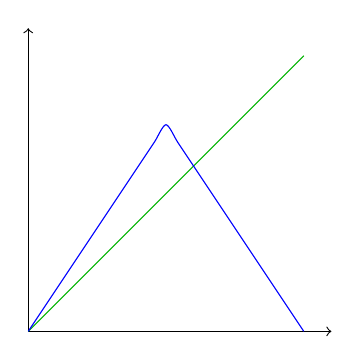
\begin{tikzpicture}[scale=3.5,declare function={f(\x)=1.5*min(\x, 1-\x);}]
	  \draw[<->](0,1.1)|-(1.1,0);
	  \draw[green!70!black] (0,0)--(1,1);
	  \draw[blue, domain=0:1, smooth] plot (\x,{f(\x)});
	\end{tikzpicture}
	\caption{$c=1.5$}
  \end{subfigure}
  \caption{Grafi $T_c$ za različne vrednsoti $c$}
  \label{fig:ds-02-tc}
\end{figure}

Poglejmo si še, kaj se zgodi z $2$-cikli.
Pri $c \le 1$ je situacija praktično enaka kot za fiksne točke, pri $c > 1$ pa
se zgodi nekaj bolj zanimivega.

\begin{figure}[h]
  \centering
  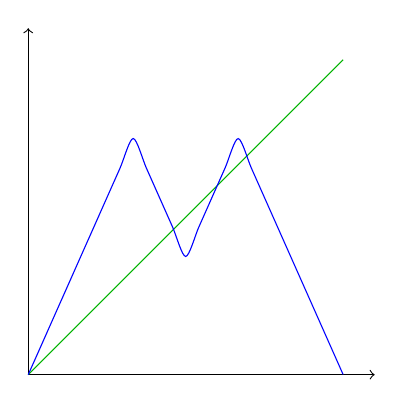
\begin{tikzpicture}[scale=4,declare function={f(\x)=1.5*min(\x, 1-\x);}]
	\draw[<->](0,1.1)|-(1.1,0); \draw[green!70!black] (0,0)--(1,1); \draw[blue,
	domain=0:1, smooth] plot (\x,{f(f(\x))});
  \end{tikzpicture}
  \caption{Graf $T_{1.5}^2$}
  \label{fig:ds-02-tc-2}
\end{figure}

V splošnem za to družino velja, da se pri večjih $c$ pojavljajo $m$-cikli, ki
postanejo gosti pri $c = 2$.
Pri $c = 1$ se zgodi tudi sprememba, da iz točke $x = \pol$ dobimo ne le odbojno
točko, ampak tudi dodaten $2$-cikel.
Točkam, pri katerih se zgodi \enquote{kvalitativna sprememba} dinamike, pravimo
\pojem{bifurkacije}.

Mi bomo bifurkacije opazovali na družinah zveznih funkcij $f_c: I \to I$, ki
bodo gladko odvisne od parametra $c \in J \subseteq \R$.
To pomeni, da za funkcijo $F(x, c) = f_c(x)$ obstajajo vsi parcialni odvodi
$\frac{\partial^k}{\partial c^k} F(x,c)$ za $k \in \N$.

Ključna opazka z motivacije je, da so se vse spremembe dinamike zgodile, ko je
bil odvod v fiksni (oz.~periodični) točki bodisi $1$ bodisi ni obstajal.
To formalizira spodnji izrek.

\begin{izrek}
  Naj bo $f_c: I \to I$ družina zvezno odvedljivih funkcij, ki so gladko odvisne
  od parametra $c \in J$.
  Denimo, da za $x_0 \in I$ velja $f_{c_0}(x_0) = x_0$ in $f_{c_0}'(x_0) \ne 1$.
  Potem obstajata okolici $I' \subseteq I$ in $J' \subseteq J$ ter preslikava
  $p: J' \to I'$, da je $f_c(p(c)) = p(c)$, za katero je $p(c)$ edina fiksna
  točka $f_c$ na $I'$.
\end{izrek}

\begin{proof}
  Uporabimo izrek o implicitni funkciji za $F(x,c) = f_c(x) - x$.
  Po predpostavki je $F(x_0, c_0) = 0$ in $\partial_x F(x_0, c_0) =
  f'_{c_0}(x_0) - 1 \ne 0$, torej lahko na majhni okolici $c_0$ izrazimo $x =
  p(c)$ ter velja $F(p(c), c) = 0$.
\end{proof}

\begin{posledica}
  Privlačne in odbojne točke so stabilne za majhne motnje, prav tako pa tudi
  točke, v katerih je odvod enak $-1$.
\end{posledica}

\begin{opomba}
  Izrek podaja le potreben, ne pa tudi zadosten pogoj.
\end{opomba}

\begin{primer}[Tangentna bifurkacija]
  To je bifurkacija, v kateri iz nevtralne točke dobimo dve fiksni točki, ki jih
  prej ni bilo.
  Ena je privlačna, druga odbojna, zato se angleško imenuje tudi
  \textit{saddle-node bifurcation}.
  Primer tega je $q_c(x) = x^2 + c$ pri $c = \inv{4}$.
\end{primer}

\begin{primer}[Potrojitev fiksne točke]
  Za $f_c(x) = c \arctan(x)$ imamo pri $c \le 1$ natanko eno fiksno točko pri $x
  = 0$, ki je privlačna za $c < 1$, pri $c = 1$ pa nevtralna in šibko privlačna.
  Pri $c > 1$ dobimo tri fiksne točke.
\end{primer}

\begin{primer}[Podvojitev periode]
  Naj bo $f_{c_0}(x_0) = x_0$ in $f_{c_0}'(x_0) = -1$.
  Po izreku se fiksna točka ohrani, za drugi $f_{c_0}^2$ pa velja
  $(f_{c_0}^2)'(x_0) = 1$, torej se lahko zgodi bifurkacija.
  Če se zgodi, potem iz fiksne točke dobimo eno fiksno točko in $2$-cikel
  (fiksne točke namreč ne moremo izgubiti in ne moremo dobiti).
  Primer take presliakve je $q_c(x) = x^2 + c$ pri $c = -\frac{3}{4}$.
\end{primer}

% LocalWords:  predperiodične Devaney Podvojitvena Konjugacije semikonjugacije
% LocalWords:  semikonjugirana semikonjugirani podvojitvena semikonjugacija
% LocalWords:  Bairovem Bifurkacije predfiksne bifurkacije bifurkacija
